\section{Теоретическая информация}
\subsection{Поверхность потенциальной энергии}
Теоретической моделью для описания химических процессов является поверхность потенциальной энергии (ППЭ). Понятие ППЭ вводится в рамках приближения Борна-Оппенгеймера, в котором предполагается, что в связи с сохранением импульса молекулярной системы и существенным превышением массы ядра над массой электрона, атомные ядра покоятся в сравнении с "быстрыми" электронами. Таким образом, электроны мгновенно подстраиваются под любое изменение ядер, и можно разделять движение электронов и ядер. В данном приближении под ППЭ понимают энергию молекулярной системы, равную \textit{сумме энергии электронов (одно- и двуэлектронные интегралы) при данной конфигурации ядер и энергии кулоновского отталкивания ядер}, записанную как функцию координат ядер $E(\vec{R})$. 

Для анализа характеристик ППЭ используют матрицу первых производных энергии по координатам ядер (градиент энергии):
\mequation{
    \left(
        \frac{\partial E}{\partial q_1}, \frac{\partial E}{\partial q_2}, \ldots, \frac{\partial E}{\partial q_{3N - 6}}  
    \right)
}
где $N$ - число атомов в системе, $\{q_i\}_{i=1}^{3N-6}$ - нормальные координаты.

Те точки, в которых все компоненты градиента равны нулю, называют критическими точками. Это могут могут быть минимумы, максимумы или седловые точки. 

Для определения типа критической точки необходимо знать матрицу вторых производных энергии по координатам ядер (матрица Гессе, гессиан):
\mequation{
    H_{ij} = \left( \frac{\partial^2 E}{\partial q_i \partial q_j} \right)
}

Если все собственные числа \textbf{H} положительны, то критическая точка является минимумом (глобальным или локальным). В случае если одно из собственных чисел \textbf{H} отрицательно, то критическая точка является седловой точкой первого порядка. Количество отрицательных собственных чисел \textbf{H} определяет порядок седловой точки.

\subsection{Методы поиска седловых точек}
В настоящее время существует ряд методов поиска седловых точек:
\begin{enumerate}
    \item требующие начального приближения для переходного состояния;
    \item требующие угадывания реакционных координат (relaxed scan);
    \item требующие угадывания реагентов и продуктов реакции (nudged elastic band method, string method, growing string method);
    \item не требующие угадывания и следующие реакциям вида $A \leftrightarrow X(+Y)$ для локального минимума A (ADDF);
    \item не требующие угадывания и следующие реакциям вида $A + B \leftrightarrow X(+Y)$ для нескольких реагентов A и B (AFIR).
\end{enumerate}

В данной работе будет использован первый подход.

\begin{figure}[H]
\centering
\captionsetup{justification=centering}
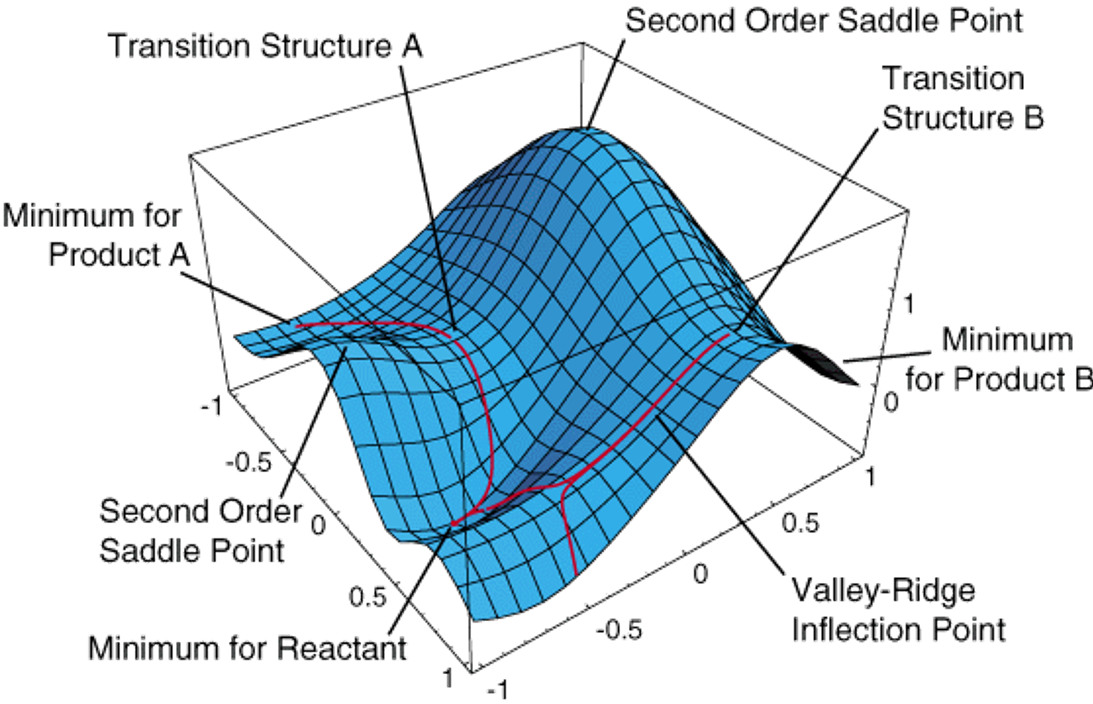
\includegraphics[scale=0.8]{fig/2.png}
\caption{ППЭ и важный точки на ней.}
\end{figure}
    